% Options for packages loaded elsewhere
\PassOptionsToPackage{unicode}{hyperref}
\PassOptionsToPackage{hyphens}{url}
\PassOptionsToPackage{dvipsnames,svgnames,x11names}{xcolor}
\PassOptionsToPackage{space}{xeCJK}
\documentclass[
  10pt,
]{article}
\usepackage{xcolor}
\usepackage[margin=0.7in]{geometry}
\usepackage{amsmath,amssymb}
\setcounter{secnumdepth}{-\maxdimen} % remove section numbering
\usepackage{iftex}
\ifPDFTeX
  \usepackage[T1]{fontenc}
  \usepackage[utf8]{inputenc}
  \usepackage{textcomp} % provide euro and other symbols
\else % if luatex or xetex
  \usepackage{unicode-math} % this also loads fontspec
  \defaultfontfeatures{Scale=MatchLowercase}
  \defaultfontfeatures[\rmfamily]{Ligatures=TeX,Scale=1}
\fi
\usepackage{lmodern}
\ifPDFTeX\else
  % xetex/luatex font selection
  \setmainfont[]{Arial}
  \setmonofont[]{Consolas}
  \ifXeTeX
    \usepackage{xeCJK}
    \setCJKmainfont[]{Microsoft YaHei}
  \fi
  \ifLuaTeX
    \usepackage[]{luatexja-fontspec}
    \setmainjfont[]{Microsoft YaHei}
  \fi
\fi
% Use upquote if available, for straight quotes in verbatim environments
\IfFileExists{upquote.sty}{\usepackage{upquote}}{}
\IfFileExists{microtype.sty}{% use microtype if available
  \usepackage[]{microtype}
  \UseMicrotypeSet[protrusion]{basicmath} % disable protrusion for tt fonts
}{}
\makeatletter
\@ifundefined{KOMAClassName}{% if non-KOMA class
  \IfFileExists{parskip.sty}{%
    \usepackage{parskip}
  }{% else
    \setlength{\parindent}{0pt}
    \setlength{\parskip}{6pt plus 2pt minus 1pt}}
}{% if KOMA class
  \KOMAoptions{parskip=half}}
\makeatother
\usepackage{longtable,booktabs,array}
\usepackage{calc} % for calculating minipage widths
% Correct order of tables after \paragraph or \subparagraph
\usepackage{etoolbox}
\makeatletter
\patchcmd\longtable{\par}{\if@noskipsec\mbox{}\fi\par}{}{}
\makeatother
% Allow footnotes in longtable head/foot
\IfFileExists{footnotehyper.sty}{\usepackage{footnotehyper}}{\usepackage{footnote}}
\makesavenoteenv{longtable}
\usepackage{graphicx}
\makeatletter
\newsavebox\pandoc@box
\newcommand*\pandocbounded[1]{% scales image to fit in text height/width
  \sbox\pandoc@box{#1}%
  \Gscale@div\@tempa{\textheight}{\dimexpr\ht\pandoc@box+\dp\pandoc@box\relax}%
  \Gscale@div\@tempb{\linewidth}{\wd\pandoc@box}%
  \ifdim\@tempb\p@<\@tempa\p@\let\@tempa\@tempb\fi% select the smaller of both
  \ifdim\@tempa\p@<\p@\scalebox{\@tempa}{\usebox\pandoc@box}%
  \else\usebox{\pandoc@box}%
  \fi%
}
% Set default figure placement to htbp
\def\fps@figure{htbp}
\makeatother
\setlength{\emergencystretch}{3em} % prevent overfull lines
\providecommand{\tightlist}{%
  \setlength{\itemsep}{0pt}\setlength{\parskip}{0pt}}
\usepackage{bookmark}
\IfFileExists{xurl.sty}{\usepackage{xurl}}{} % add URL line breaks if available
\urlstyle{same}
\hypersetup{
  colorlinks=true,
  linkcolor={Maroon},
  filecolor={Maroon},
  citecolor={Blue},
  urlcolor={blue},
  pdfcreator={LaTeX via pandoc}}

\author{}
\date{}

\usepackage{float}
\usepackage{needspace}
\Urlmuskip=0mu plus 2mu\relax
\renewcommand{\figurename}{图}
\begin{document}

\section{新数据集与眼底图像退化实验：进度总览}\label{ux65b0ux6570ux636eux96c6ux4e0eux773cux5e95ux56feux50cfux9000ux5316ux5b9eux9a8cux8fdbux5ea6ux603bux89c8}

2026 年 11 月 13 日 · \href{progress-overview.en.md}{English} ·
\href{progress-overview.zh.pdf}{PDF}

项目已完成本轮公开数据审查、新增图像的标签和关联核验、训练数据划分，以及四组青光眼分类实验。扩展数据显著改善了
KEH 和 LAG 开发集的图像排序；在合成失焦条件下，50\%
退化增强提高了排序表现并减少误报，同时增加了阈值 0.5
下的阳性漏诊。下一轮工作重点是保持原来源的训练采样量、改进模型选择规则，并补充真实低质量阴性病例。分类阈值、质量引导的人工复核规则及最终测试尚待完成。

本目录按实验顺序组织为\href{data-review/data-and-degradation-review.zh.md}{数据与方法审查}、\href{training-results/training-results.zh.md}{训练结果}和\href{experimental-analysis/experimental-analysis.zh.md}{统计分析}。三份报告记录同一天工作的不同阶段。本总览以完成训练后的数据版本和第
1,200 次更新权重为准。

\subsection{数据准备完成了什么}\label{ux6570ux636eux51c6ux5907ux5b8cux6210ux4e86ux4ec0ux4e48}

公开来源审查覆盖 45 个数据集或数据集系列。逐图核验后，新增池纳入 9,070
张图像，包括 3,446 张阳性图像；另有 204
张疑似图像单列记录。阳性标签保留各来源的原始定义，其中 3,443
张为来源定义的青光眼阳性，3 张为 AIROGS
的转诊阳性。视盘裁剪图与完整眼底照片分别标记。

新增池经关联分组后，与修正后的原数据组成 24,491
张图像的疾病训练与评价清单。原训练与验证部分中，18 张关联官方 EyeQ
测试图像的照片已移除；规则开发部分沿用身份关联核查后的 1,220 张原图。

\Needspace{8\baselineskip}
\begin{longtable}[]{@{}lrrr@{}}
\toprule\noalign{}
用途 & 修正后原数据 & 新增数据 & 合计 \\
\midrule\noalign{}
\endhead
\bottomrule\noalign{}
\endlastfoot
疾病模型训练 & 10,338 & 5,142 & 15,480 \\
模型验证 & 1,188 & 858 & 2,046 \\
人工复核规则开发 & 1,220 & 833 & 2,053 \\
内部及新增保留测试 & 1,233 & 2,237 & 3,470 \\
ACRIMA 外部测试 & 705 & 0 & 705 \\
HYGD 外部测试 & 737 & 0 & 737 \\
\end{longtable}

训练集含 6,405 张阳性，模型验证集含 823 张阳性，规则开发集含 814
张阳性。已知患者和确认的关联图像按组分配用途。PAPILA
整个纳入来源用于保留测试，FIVES 和 Fundus-AVSeg 的官方测试角色保留。全部
24,491 张图像通过文件哈希及完整 RGB 解码核验。

\begin{figure}[H]
\centering
\pandocbounded{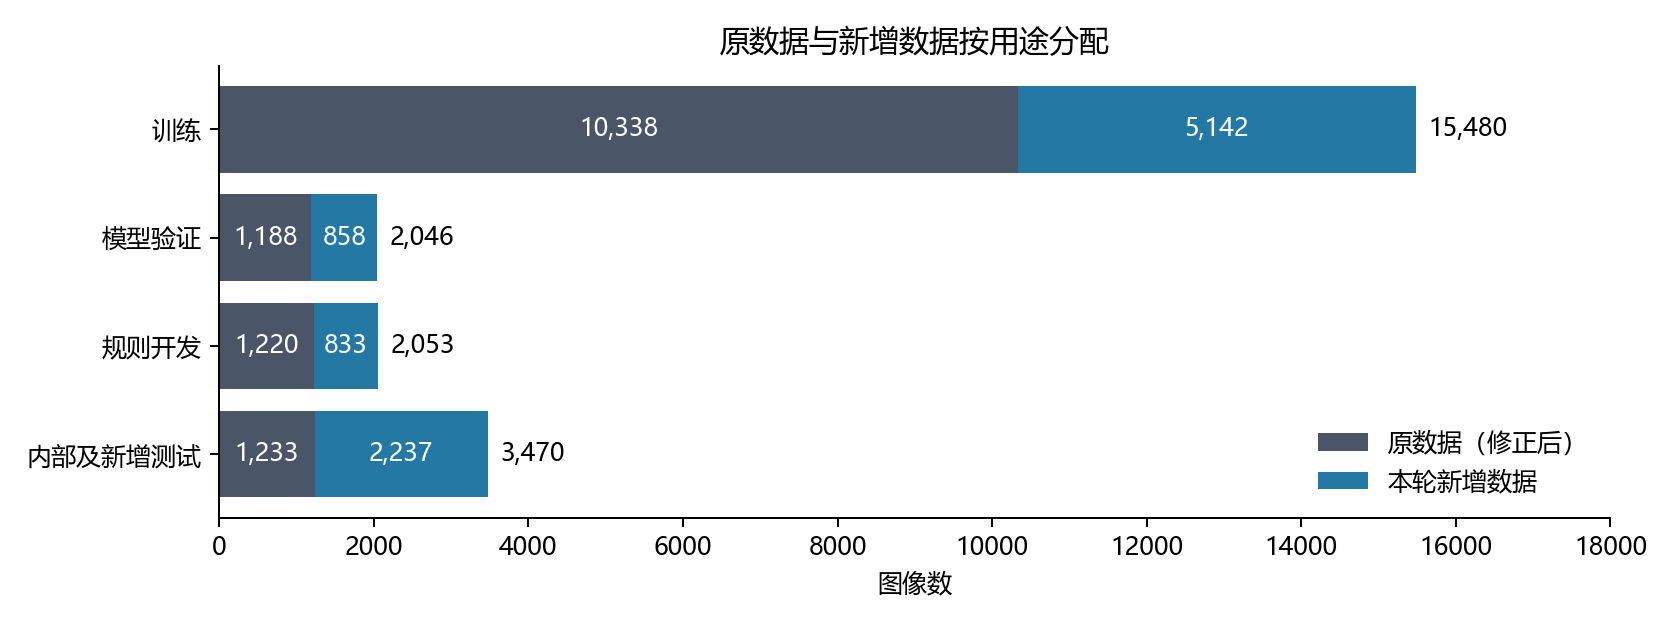
\includegraphics[keepaspectratio,alt={原数据和新增图像按用途分配}]{cohort-allocation.zh.png}}
\caption{原数据和新增图像按用途分配}
\end{figure}

图 1 显示四项主要用途的数据组成；数字为原图数量。新增池的 5,142
张图像进入训练，其余进入模型验证、规则开发或保留测试。ACRIMA 和 HYGD
合计 1,442 张外部测试图另列于表中。

\subsection{本轮实验如何比较}\label{ux672cux8f6eux5b9eux9a8cux5982ux4f55ux6bd4ux8f83}

四组均使用 EfficientNet-B0、相同初始化和随机种子 20261113，每批最多 16
张图像，各完成 1,200 次优化更新。原数据组使用修正后的 10,338
张训练图像，其余三组使用 15,480 张。扩展数据分别配合 0\%、30\% 和 50\%
的混合退化应用概率，退化包括照明不均、失焦和散射。质量模型的监督目标沿用原图，退化增强用于疾病模型训练。

模型每 300 次更新在共同的 2,046 张模型验证图像上评价。原选模规则对 11
个含正负两类的来源等权平均 AUROC。原数据、30\% 和 50\%
退化组的选中权重均来自第 1,200 次更新，扩展无退化组来自第 300
次更新。下面统一比较第 1,200 次更新，便于判断相同训练预算下的差异。

\subsection{已观察到的结果}\label{ux5df2ux89c2ux5bdfux5230ux7684ux7ed3ux679c}

AUROC
的全称是``受试者工作特征曲线下面积''。模型输出疾病分数，改变判为阳性的分数阈值，可以得到一系列敏感度（检出的阳性比例）和误报率（被判为阳性的阴性比例）；ROC
曲线展示两者的关系，AUROC 是曲线下的面积。

它也可以理解为：随机抽取一张阳性和一张阴性图像，模型给阳性更高分的概率，并列分数计一半。例如
AUROC 为 0.93 表示这一排序概率约为 93\%；0.5 相当于随机排序，1.0
表示完全区分。实际漏诊和误报需在选定阈值下另行评价。下表来自同一规则开发集的原图，各来源独立计算。

\Needspace{8\baselineskip}
\begin{longtable}[]{@{}lrrrr@{}}
\toprule\noalign{}
来源 & 原数据 & 扩展数据 & 30\% 退化 & 50\% 退化 \\
\midrule\noalign{}
\endhead
\bottomrule\noalign{}
\endlastfoot
AIROGS & 0.9687 & 0.9551 & 0.9583 & 0.9593 \\
ODIR & 0.9712 & 0.9315 & 0.9281 & 0.9404 \\
LAG & 0.9465 & 0.9890 & 0.9844 & 0.9832 \\
KEH & 0.6627 & 0.9333 & 0.9321 & 0.9368 \\
\end{longtable}

各来源开发图像数／阳性数分别为 AIROGS 773／380、ODIR 305／28、LAG
481／169、KEH 153／75。

扩展相对原数据的 AUROC 差，在 KEH 为 +0.2706，在 LAG 为
+0.0425；按关联组进行 4,000 次配对重采样所得的 95\% 区间分别为
{[}0.1818, 0.3639{]} 和 {[}0.0248, 0.0616{]}。AIROGS 和 ODIR 分别下降
0.0136 和
0.0397，对应区间均低于零。这些区间表示开发病例抽样的不确定性；本轮使用一个训练种子。

压力评价对固定的 384 张规则开发原图生成失焦和曝光降低变体，包括 146
张阳性和 238 张阴性。50\% 退化相对扩展无退化，在失焦条件下的 AUROC 从
0.8894 提高到 0.9449；阈值 0.5 下误报由 68/238 降至 19/238，漏诊由
18/146 升至
28/146。固定模型验证集设定的来源阈值后，误报减少与漏诊增加的方向一致。

\begin{figure}[H]
\centering
\pandocbounded{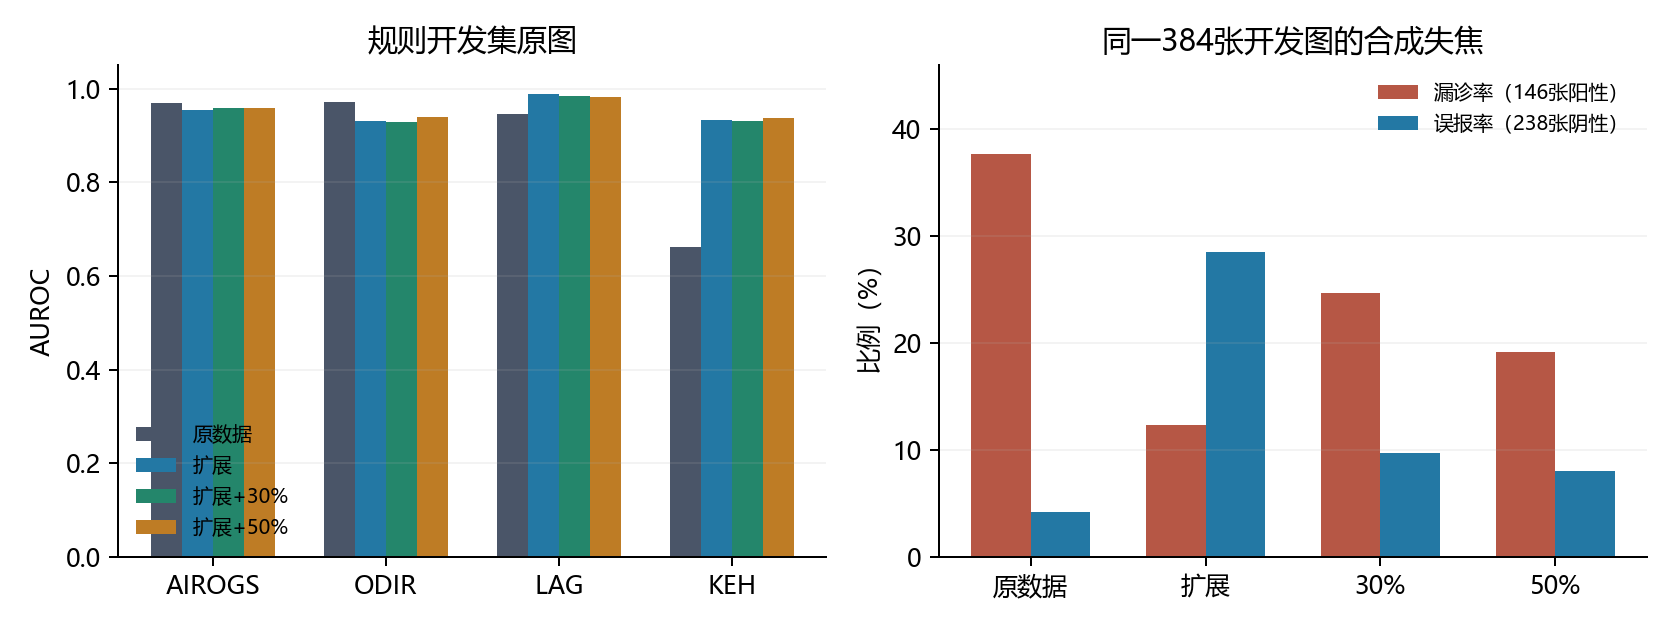
\includegraphics[keepaspectratio,alt={第1200次更新的来源排序与合成失焦结果}]{experiment-overview.zh.png}}
\caption{第1200次更新的来源排序与合成失焦结果}
\end{figure}

图 2 左侧展示四个来源的原图 AUROC，右侧展示同一失焦开发子集在阈值 0.5
下的漏诊率和误报率。右侧两项比例分别以阳性和阴性图像数为分母。退化增强的作用需同时结合排序、漏诊和误报评价。

真实低质量开发病例为 FIVES 的 7 张和 MSHF 的 5 张阳性图像。在阈值 0.5
下，原数据组检出 7/12，三个扩展组均检出 12/12；12/12 的二项分布 95\%
区间为
73.5\%--100\%。该子集全部为阳性，且三个扩展组的检出数一致，因此本轮的真实低质量检出改善主要体现在数据扩展。后续需结合相同来源的阴性图像评价误报。

\subsection{分析指出的下一步}\label{ux5206ux6790ux6307ux51faux7684ux4e0bux4e00ux6b65}

扩大训练池后，原来源图像的累计采样次数由 19,186 降为
9,484；三个扩展组使用相同的图像采样序列。新增来源适应与原来源采样量变化同时发生，下一轮将用原来源采样配额区分两者作用。

现有选模平均值中，HRF、CRFO、Fundus-AVSeg 和 LES-AV 合计只有 15
张验证图像，却占四个等权来源，即 36.4\%
的权重。这使少数图像的排序变化明显影响权重选择。下一轮拟以
AIROGS、ODIR、Kaggle、LAG 和 KEH
为主要选模来源，保存每次验证权重，并采用三个共同随机种子与 2,400
次更新预算。

真实低质量训练图像的质量标记与疾病类别高度相关。后续还需补充真实低质量阴性图像，分别比较失焦增强与混合退化，并在模型验证数据上设定分类阈值。完成这些比较后，选择疾病模型和质量模型、开发人工复核规则，固定规则再评价保留测试集。详细实验安排见\href{experimental-analysis/experimental-analysis.zh.md}{统计分析}与\href{../../operations/next-steps.md}{下一步清单}。

\subsection{与此前训练的关系及证据}\label{ux4e0eux6b64ux524dux8badux7ec3ux7684ux5173ux7cfbux53caux8bc1ux636e}

此前 \texttt{formal\_v3} 两套疾病模型、原质量模型和
\texttt{eyeq\_quality\_v1} 均已完成 20 轮训练。11 月 12
日报告记录的疾病权重选自第 16 和 18 轮，在 AIROGS 模型验证集上的 AUROC
为 0.9766 和 0.9831；EyeQ 质量模型选中第 17 轮权重，在 117 张 EyeQ
验证图像上的三档 macro-F1 为 0.811。本轮固定 1,200
次更新实验采用新的数据清单，评价集也已扩展；两轮结果分别解释。

可核查的证据包括\href{../../../data/prepared/expanded_20261113/cohort_verification.json}{冻结清单核验}、\href{../../../runs/expanded_20261113/budget_end_comparison.json}{第
1,200
次更新结果}、\href{experimental-analysis/analysis.json}{配对统计}及\href{../../../tools/build_progress_overview_20261113.py}{报告构建程序}。逐图预测、完整训练日志、数据文件与模型权重位于本地数据和运行目录；报告中的汇总表、图和统计结果随仓库保存。

\end{document}
